\documentclass{article}
\usepackage{fancyhdr}
\usepackage[utf8]{inputenc}
\usepackage[english]{babel}
\usepackage{tikz, multicol, graphicx, etoolbox, enumerate, setspace, relsize, mathrsfs, verbatim}
\usepackage{amsmath, amsfonts, amssymb, amsthm, epsfig, epstopdf, titling, url, array, esvect, tikz-3dplot}
\usepackage{graphicx}
\usepackage{hyperref}

\usepackage{listings}
\usepackage{xcolor}

\definecolor{codegreen}{rgb}{0,0.6,0}
\definecolor{codegray}{rgb}{0.5,0.5,0.5}
\definecolor{codepurple}{rgb}{0.58,0,0.82}
\definecolor{backcolour}{rgb}{0.95,0.95,0.92}


\usepackage{pgfplots}
\usepackage{tcolorbox}
\usepackage{amsthm}
\usepackage{cancel}
\usepackage[left=1in,right=1in,top=1in,bottom=1in]{geometry}
\usepackage[tableaux]{prooftrees}

\lstdefinestyle{mystyle}{
    backgroundcolor=\color{backcolour},   
    commentstyle=\color{codegreen},
    keywordstyle=\color{magenta},
    numberstyle=\tiny\color{codegray},
    stringstyle=\color{codepurple},
    basicstyle=\ttfamily\footnotesize,
    breakatwhitespace=false,         
    breaklines=true,                 
    captionpos=b,                    
    keepspaces=true,                 
    numbers=left,                    
    numbersep=5pt,                  
    showspaces=false,                
    showstringspaces=false,
    showtabs=false,                  
    tabsize=2
}

\lstset{style=mystyle}

\pagestyle{fancy}
\fancyhf{}
\fancyhead[L,RO]{Tasksheet 4}
\fancyhead[R,RO]{Fundamentals of Computational Mathematics}
\fancyfoot[L,RO]{Xiang Gao}
\fancyfoot[R,RO]{Math 4610}
\renewcommand{\headrulewidth}{0.4pt}% Default \headrulewidth is 0.4pt
\renewcommand{\footrulewidth}{0.4pt}% Default \footrulewidth is 0pt
\def\checkmark{\tikz\fill[scale=0.4](0,.35) -- (.25,0) -- (1,.7) -- (.25,.15) -- cycle;} 

\begin{document}

\section*{Task 1}
I have created a absErr.py file and relErr.py file each with their own testing file. I have documented both .py files in my Software Manual. In addition, I have added the error files to my shared library.\\
The routine for the absolute error is provided below:
\lstinputlisting[language=Python]{absErr.py}
With the following code for testing:
\lstinputlisting[language=Python]{test_absErr.py}
And the following output:
\begin{center}
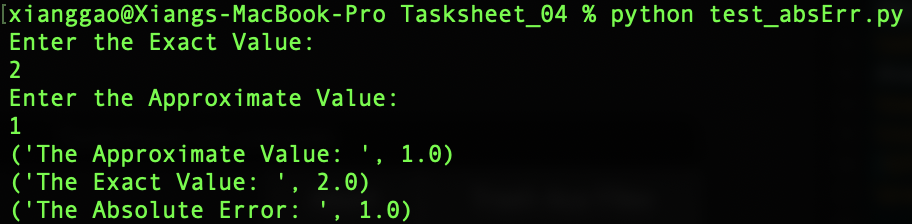
\includegraphics[width=\textwidth]{Screenshots/test_absErr.png}
{\bf Figure 1.} Machine Epsilon Single Precision Output:
\end{center}
The routine for relative error is provided below:
\lstinputlisting[language=Python]{relErr.py}
With the following code for testing:
\lstinputlisting[language=Python]{test_relErr.py}
And the following output:
\begin{center}
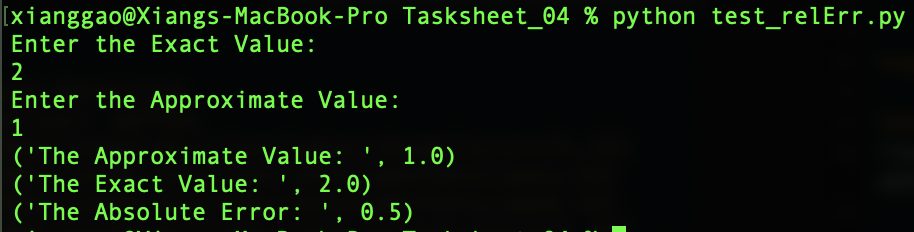
\includegraphics[width=\textwidth]{Screenshots/test_relErr.png}\\
{\bf Figure 2.} Machine Epsilon Double Precision Output.
\end{center}

\vspace{5pt}

\section*{Task 2}
I have created a graphics routine as shown in the following:
\lstinputlisting[language=Python]{graphicsRoutine.py}
Where I wanted to draw the {\bf topologist's sine wave}, so I give it the following input
\begin{center}
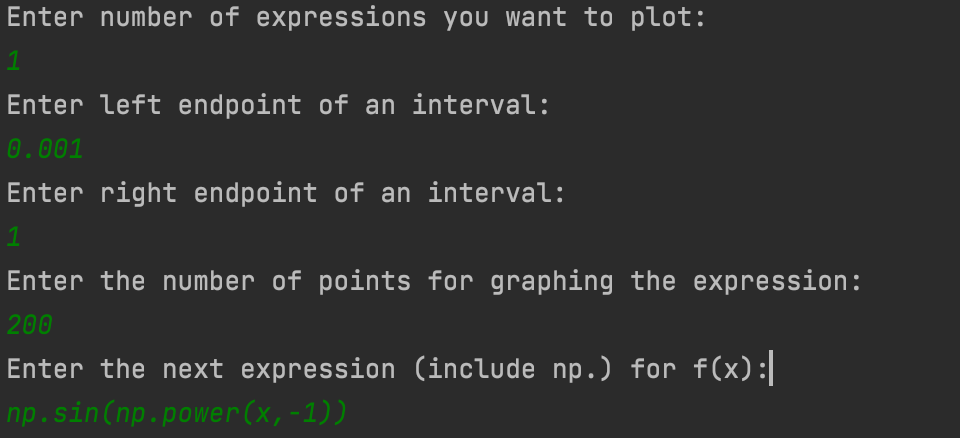
\includegraphics[scale = 0.8]{Screenshots/input.png}\\
{\bf Figure 3.} Input for the Graphics Routine.
\end{center}
And it produced the following output
\begin{center}
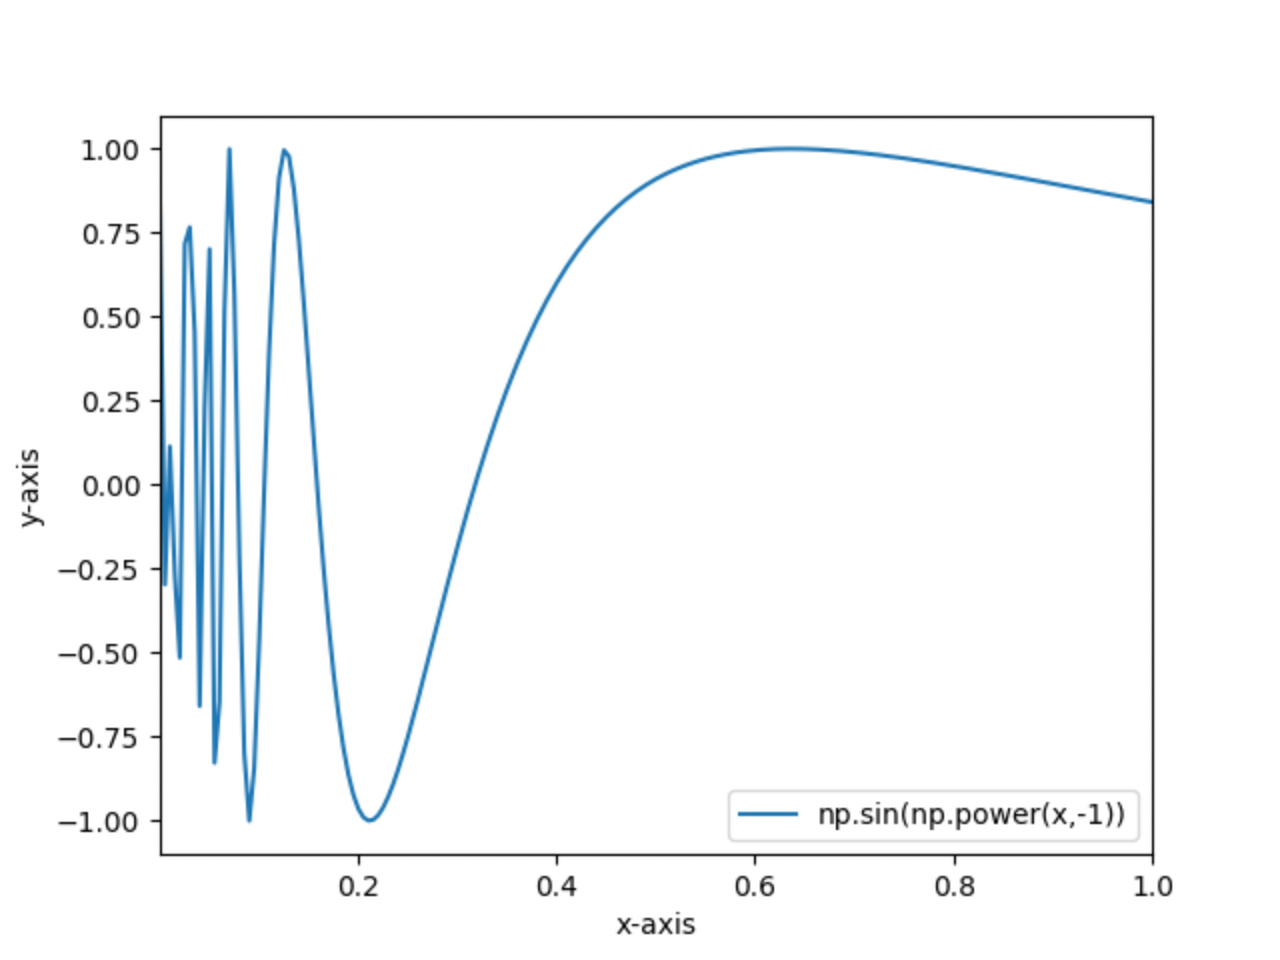
\includegraphics[scale = 0.52]{Screenshots/output.png}\\
{\bf Figure 4.} Output for the Graphics Routine.
\end{center}

\vspace{5pt}

\section*{Task 3}
The routine is given by the following:
\lstinputlisting[language=Python]{Task_3.py}
And the result is given by:
\begin{center}
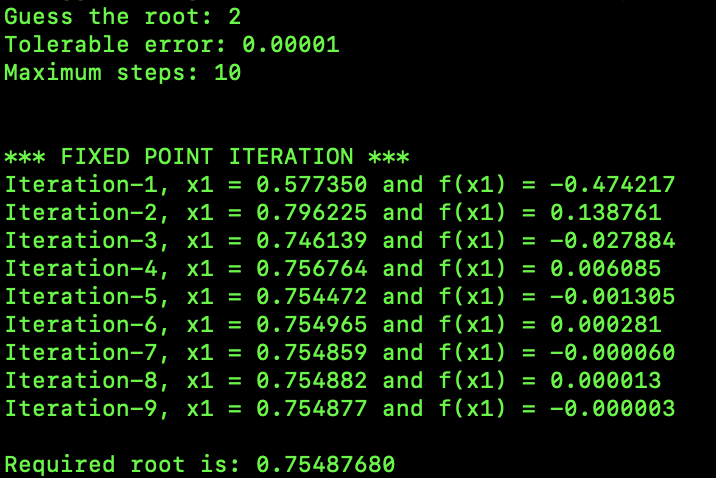
\includegraphics[scale = 1]{Screenshots/fixedPoints.png}\\
{\bf Figure 5.} Fixed point method for an example function.
\end{center}

\section*{Task 4}
Use the code for the previous task, I got the following result.
\begin{center}
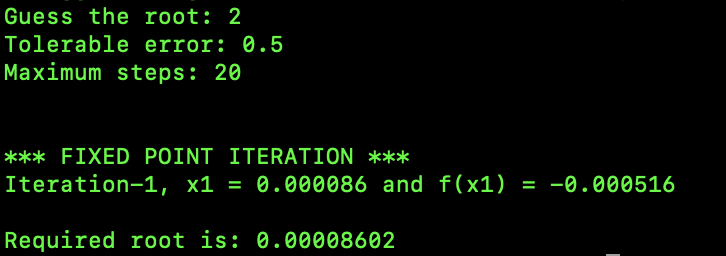
\includegraphics[scale = 0.8]{Screenshots/Task4.png}\\
{\bf Figure 6.} Fixed point method for $f(x) = xe^{3x^2} - 7x$.
\end{center}

\section*{Task 5}
The routine is given by the following:
\lstinputlisting[language=Python]{Task_5.py}
And the result is given by:
\begin{center}
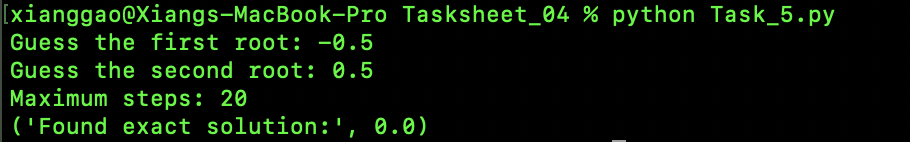
\includegraphics[width=\textwidth]{Screenshots/5.png}\\
{\bf Figure 7.} Bisection method for $f(x) = xe^{3x^2} - 7x$.
\end{center}


\section*{Task 6}
From this \href{https://math.stackexchange.com/questions/29197/applied-math-finding-roots}{website}\footnote{https://math.stackexchange.com/questions/29197/applied-math-finding-roots} I found, I realize that root finding methods are important when we can't find a root for a really complicated system, and finding them numerically is sometimes are our best shot. \\
There are also different kinds of \href{https://www.jenkins.io/doc/book/pipeline/shared-libraries/}{shared libraries}\footnote{https://www.jenkins.io/doc/book/pipeline/shared-libraries/}. For examples:
	\begin{enumerate}
		\item Static Libraires;
		\item Global Shared Libraries;
		\item Folder-level Shared Libraries;
		\item Automatic Shared Libraries
	\end{enumerate}
The pro of static libraries is its simplicity, however, you are bounded to program statically (doesn't really know what it means, but it sounds like a con).

\end{document}